\chapter{E-learning jako přenos informace}

V této kapitole se čtenář seznámí s několika základními definicemi pojmu e-learning, dozví se, jak se běžně na tento jev nahlíží. Seznámí se s některými pro a proti nasazení e-learningu jakožto výukového média a média pro získávání a předávání informace.

Dále bude čtenáři poskytnut vhled do současného trendu využití e-learningu v herním průmyslu a naopak, využití herního průmyslu v procesu e-learningu. 

Čtenář se také dozví o vzniku fenoménu GWAP (Game With a Purpose), jeho praktickém užití a některých příkladech zapracování do života běžného uživatele webu.

Nakonec bude zmíněn vztah GWAP modelu a hry \verb|trogASR|.

\section{Co je to e-learning}

Definovat e-learning (\nom{EL}{E-Learning}) se může zdát úkolem poněkud obtížným, jelikož žádná jedna konkrétní definice nepostihne všechny oblasti a aspekty EL. Proto je zde uvedeno několik definic a ponecháno na čtenáři, nechť si vybere tu pro něj nejpříhodnější.

\begin{itemize}
\item \uv{EL je výuka s využitím výpočetní techniky a internetu} \cite{korviny_2005}.
\item \uv{EL je způsob provozu výuky, tréninku, či edukačního programu pomocí elektronických prostředků. EL zahrnuje využití počítače, nebo jiného elektronického zařízení (například mobilního telefonu), jako média pro poskytnutí tréninkového, edukativního, či učebního materiálu} \cite{stockley_2003}.
\item \uv{EL je takový typ učení, při němž získávání a používání znalostí je distribuováno a usnadňováno elektronickými zařízeními} \cite{prucha_2009}.
\end{itemize}

\subsection{Proč používat e-learning}

Jak \cite{fongling_2006} podotýká, tradiční studenti jsou při procesu EL více spontánní a otevření. Většinou si jsou schopni nalézt vlastní postup organizace výuky, který je pro ně nejméně násilný a může být tedy výrazně efektivnější, než-li způsoby výuky v kamenné třídě s figurou absolutního supervizora -- učitele.

EL přináší další výhody oproti klasickým výukovým metodám. Díky dostupnosti virtuálních médií mohou žáci sedět na druhém konci světa a studovat kurzy expertů, se kterými by se jen těžce osobně setkávali.

EL skrz webové rozhraní přináší o to lepší možnost rozšiřitelnosti; web jako takový využívá v dnešní době naprostá většina civilizovaného světa. Má tedy smysl využívat právě toto médium jako to dominantní.

EL je dostupný v dnešní době každému a kdykoli; odpadá závislost na fyzickém kontaktu dvou osob pro průběh procesu předání informace. Tento fakt značně hraje do noty celkovému dnešnímu trendu, jenž míří směrem globalizace a postupného odpadávání fyzické komunikace jako takové.

EL může být masový. Běžný vyučující je schopen reálně zvládnout třídu třiceti žáků. S dobře navrženým EL systémem mohou najednou pracovat miliony lidí. A to při vytížení toho samého jednoho učitele, který daný EL kurz navrhl a realizoval.

\subsection{Proč e-learning nepoužívat}

EL jako koncept má mnoho výhod, avšak je pln i inherentních nevýhod, plynoucích povětšinou ze způsobů nasazení a podání.

Jakkoli velký může mít EL přínos pro předání informace, může mít dopad na kvalitu informace samotné. Vzděláváme-li se prostřednictvím médií a autorů, jejichž identita je skryta, informace, získaná tímto způsobem, nemusí být nutně validní. Nemusíme mít kontrolu nad zdrojem informace, nemáme páky, jak informaci verifikovat. Přesto bývá informaci, předávané virtuálně, přikládán jaksi absolutní význam.

Dalším dopadem je separace vyučujícího a vyučovaného. Nemůžeme si dostatečně jasně vymezit názor na zdroj, který nám EL program připravil. Tento údaj se může zdát nepotřebný. Je však nasnadě si uvědomit, že ač věříme svému úsudku bezmezně, šikovnou manipulací s údaji o původu zdroje lze naše podvědomí naprogramovat na zvýšenou / sníženou hladinu zájmu o poskytovaný materiál.

EL může zaviňovat i úpadek socializační. Studenti nejsou nuceni opouštět zázemí své domény a interagovat se svými vrstevníky, spolustudenty a lektory fyzicky. Stačí jim otevřít rozhraní svého konkrétního média a komunikovat jeho prostřednictvím.

\section{Výuka a počítačové hry}

\epigraph{\sl\uv{Počítačové hry mi zničily život. Ještě, že mám další dva.}}{--- autor neznámý}

Téma výuky prostřednictvím počítačových her je dnes a denně omílanou parafrází. 

Na jednu stranu, plejáda edukativních her a hříček nabízí pohled na interakci výuky a herního průmyslu jako na proces oboustranně výhodný. Student --- hráč --- je vtažen do interaktivního prostředí počítačové hry, kde může objevovat a osahat si koncepty, které v reálném světě mohou být náročné na vysvětlení, nebo v něm dokonce ani nemusí existovat \cite{graven_2006}. Herní vývojář naopak získává platícího zákazníka.

Na druhou stranu, student --- hráč --- může být vystaven vlivům nežádoucím; pro svůj věk, svou psychickou vyspělost, či pro svou víru a formování osobnosti. Násilí, nepřiměřená erotika, nespisovný a vulgární slovník mohou zapříčinit zkreslení náhledu na svět, obzvlášť u jedinců nedospělých, s ne zcela zformovanou osobností. 

Jak ale \cite{xuemin_2009} uvádí, negativní sociální dopady na hráče nezapříčiňuje často hra samotná, nýbrž prostředí, ve kterém se hráč při hraní pohybuje. Negativistické rodinné zázemí, domácí násilí, nepohoda, toto jsou stresory, které, dokresleny vulgární počítačovou hrou, mohou propuknout až v agresivní chování hráče, jeho depresivní sklony, popřípadě v inklinaci k násilí. Jak \cite{xuemin_2009} také uvádí, i násilná počítačová hra může mít pozitivní vliv na zdravého jedince a poskytnout mu nástroj k formování základních kognitivních procesů, rychlého uvažování a přístupu k řešení problémů.

S čím se často setkáváme u hráčů, hrajících počítačové hry v jazyce jiném, než je mateřský, bývá až nečekaný nárůst jazykových schopností. Tento proces u zarputilých hráčů může vést až k částečnému, nebo i úplnému, bilingvismu. Hráč má totiž zájem sám sebe vzdělávat v jazyce své oblíbené hry. Pokud nějaké frázi v daném jazyce nerozumí, rád a dobrovolně si ji vyhledá ve slovníku, aby byl schopen ve hře pokračovat \cite{bialystok_2006}.

\section{E-learning hrou a crowdsourcing}

Crowdsourcing (\nom{CS}{Crowdsourcing}), též někdy {\sl wisdom of the crowds} (moudrost davů), je označení pro způsob dělby práce, kde se pro řešení problému místo zaměstnance, či kontraktora, využije blíže nespecifikovaná skupina lidí ({\sl crowd} -- dav) v rámci všeobecné výzvy.

CS se často využívá například při vývoji nové technologie (testování), zdokonalování algoritmu (komparace výsledků), či pro zachycení, analýzu a třídění velkého množství dat.

\uv{Každý rok, lidé na celém světě stráví miliardy hodin hraním počítačových her. Co kdyby mohl tento vynaložený čas a energie být soustředěny do užitečné práce? Co kdyby lidé, hrající počítačové hry, mohli bezděky zároveň řešit rozsáhlé a náročné problémy?} \cite{ahn_2006}

Díky této otázce vzniká pojem {\sl hra s účelem} (\nom{GWAP}{Game With a Purpose} -- Game With a Purpose). Jedná se, jak název napovídá, o počítačovou hru, která mimo pobavení hráče zároveň plní jiný, taktéž smysluplný účel. Lze zde vidět krásné použití CS a EL v praxi. Uživatelé se nevědomky stávají součásti procesu CS a ještě se při tom baví a vzdělávají.

\subsection{ESP game}

\begin{figure}[h]
	\centering
	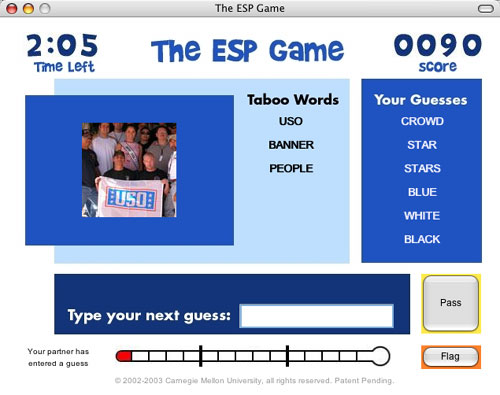
\includegraphics[width=110mm,height=80mm]{img/esp.jpg}
	\caption{Ukázka {\sl ESP game}}
	\label{fig:esp}
\end{figure}

Pojem GWAP se poprvé začal objevovat v souvislosti s \verb|ESP game| \cite{ahn_2004}. \verb|ESP game| (později \nom{GIL}{Google Image Labeler} -- Google Image Labeler) je hra vyvinutá pro popasování se s problémem vytváření komplexních metadat obrázků.

Původně měla \verb|ESP game| řešit úkol, který tou dobou stroje nezvládaly, to jest rozpoznávání obrázků. Díky tomu, že autoři zabalili tento úkol do jednoduché hry, mohli využít ohromného potenciálu zahálejících uživatelů webu.

\subsection{Duolingo}

\begin{figure}[h]
	\centering
	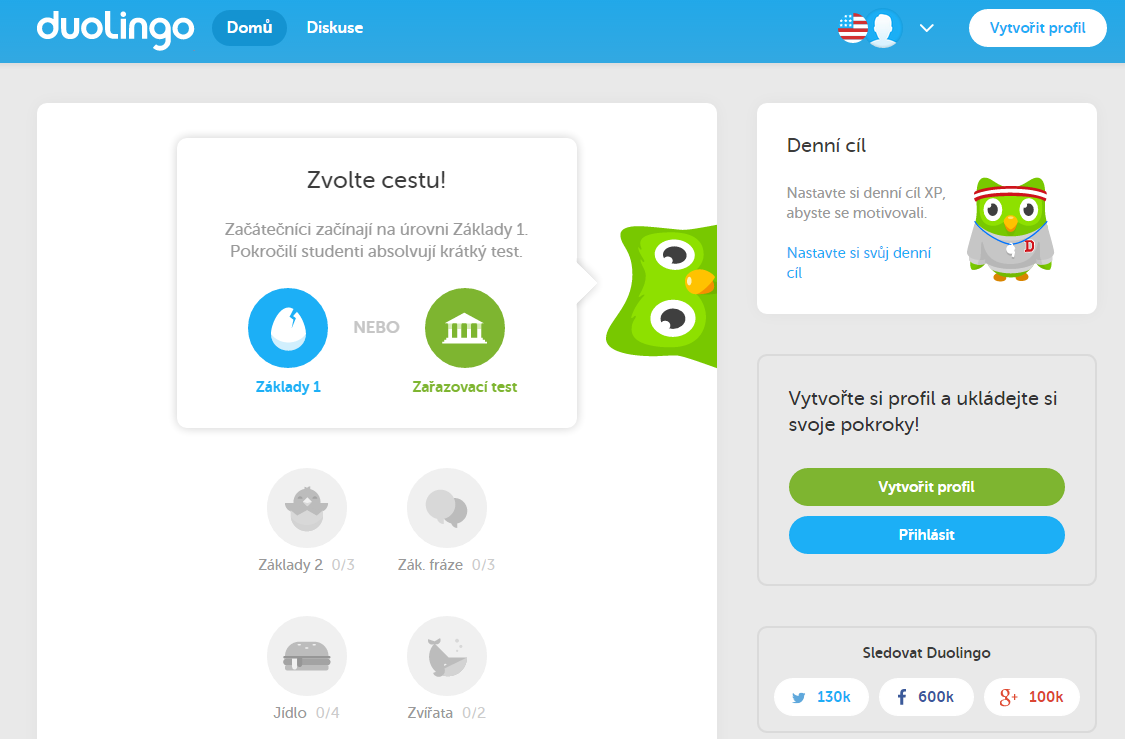
\includegraphics[width=110mm,height=80mm]{img/duolingo.png}
	\caption{Ukázka {\sl Duolingo}}
	\label{fig:duolingo}
\end{figure}

\verb|Duolingo|\footnote{\url{https://www.duolingo.com/}} je populární webová hra pro výuku jazyka. Umožňuje například soutěžit s přáteli v jazykové zdatnosti prostřednictvím sítě Facebook.

Nalezneme zde desítky jazykových kurzů, v současnosti i kurzy angličtiny pro české mluvčí. V rámci výuky jsou zde překládány texty partnerských společností, které za překlady platí. Studenti pak provádí samotný překlad a data posléze i verifikují.

\subsection{reCAPTCHA}

\begin{figure}[h]
	\centering
	
\includegraphics[width=80mm,height=20mm]{img/recaptcha.png}
	\caption{Ukázka {\sl reCAPTCHA}}
	\label{fig:recaptcha}
\end{figure}

\verb|reCAPTCHA|\footnote{\url{https://www.google.com/recaptcha/intro/index.html}} \cite{ahn_2008} není tak úplně hrou. Jedná se o dialog mezi uživatelem a počítačem, který má zjistit, zda uživatel není také stroj. Zároveň jsou tímto procesem získávána data o prezentovaných obrázcích a jejich obsahu.

Díky \verb|reCAPTCHA| procesu se podařilo například digitalizovat celý archiv {\sl New York Times}. Zároveň je takto podporován vývoj softwaru pro strojové rozpoznávání textu, který je na oplátku používán pro prolomení \verb|reCAPTCHA| kontroly.

\section{TrogASR jako GWAP}

\verb|TrogASR| aplikace, kterou tato práce reprezentuje, je bezesporu typickou GWAP. Jedná se o webovou hru s účelem jazykové výuky za pomoci soupeření o místa na žebříčku, čímž se nejvíce podobá hře \verb|Duolingo| ze zmíněných.

Na jazykovou výuku jde ale z jiného úhlu. Na rozdíl od \verb|Duolingo| nevyžaduje psaný uživatelský vstup, nýbrž vstup hlasový. Cílem tohoto návrhového kroku je poskytnout uživateli větší pocit \uv{zatažení} do hry a inteligentnější interakce.

Stran smyslu hry \verb|trogASR| lze uvést stránku EL --- uživatel projevuje a zdokonaluje své jazykové znalosti --- a stránku CS --- uživatel bezděčně poskytuje verifikovaná data \verb|CloudASR| knihovně.
